% GNUPLOT: LaTeX picture with Postscript
\begingroup
  \makeatletter
  \providecommand\color[2][]{%
    \GenericError{(gnuplot) \space\space\space\@spaces}{%
      Package color not loaded in conjunction with
      terminal option `colourtext'%
    }{See the gnuplot documentation for explanation.%
    }{Either use 'blacktext' in gnuplot or load the package
      color.sty in LaTeX.}%
    \renewcommand\color[2][]{}%
  }%
  \providecommand\includegraphics[2][]{%
    \GenericError{(gnuplot) \space\space\space\@spaces}{%
      Package graphicx or graphics not loaded%
    }{See the gnuplot documentation for explanation.%
    }{The gnuplot epslatex terminal needs graphicx.sty or graphics.sty.}%
    \renewcommand\includegraphics[2][]{}%
  }%
  \providecommand\rotatebox[2]{#2}%
  \@ifundefined{ifGPcolor}{%
    \newif\ifGPcolor
    \GPcolortrue
  }{}%
  \@ifundefined{ifGPblacktext}{%
    \newif\ifGPblacktext
    \GPblacktexttrue
  }{}%
  % define a \g@addto@macro without @ in the name:
  \let\gplgaddtomacro\g@addto@macro
  % define empty templates for all commands taking text:
  \gdef\gplbacktext{}%
  \gdef\gplfronttext{}%
  \makeatother
  \ifGPblacktext
    % no textcolor at all
    \def\colorrgb#1{}%
    \def\colorgray#1{}%
  \else
    % gray or color?
    \ifGPcolor
      \def\colorrgb#1{\color[rgb]{#1}}%
      \def\colorgray#1{\color[gray]{#1}}%
      \expandafter\def\csname LTw\endcsname{\color{white}}%
      \expandafter\def\csname LTb\endcsname{\color{black}}%
      \expandafter\def\csname LTa\endcsname{\color{black}}%
      \expandafter\def\csname LT0\endcsname{\color[rgb]{1,0,0}}%
      \expandafter\def\csname LT1\endcsname{\color[rgb]{0,1,0}}%
      \expandafter\def\csname LT2\endcsname{\color[rgb]{0,0,1}}%
      \expandafter\def\csname LT3\endcsname{\color[rgb]{1,0,1}}%
      \expandafter\def\csname LT4\endcsname{\color[rgb]{0,1,1}}%
      \expandafter\def\csname LT5\endcsname{\color[rgb]{1,1,0}}%
      \expandafter\def\csname LT6\endcsname{\color[rgb]{0,0,0}}%
      \expandafter\def\csname LT7\endcsname{\color[rgb]{1,0.3,0}}%
      \expandafter\def\csname LT8\endcsname{\color[rgb]{0.5,0.5,0.5}}%
    \else
      % gray
      \def\colorrgb#1{\color{black}}%
      \def\colorgray#1{\color[gray]{#1}}%
      \expandafter\def\csname LTw\endcsname{\color{white}}%
      \expandafter\def\csname LTb\endcsname{\color{black}}%
      \expandafter\def\csname LTa\endcsname{\color{black}}%
      \expandafter\def\csname LT0\endcsname{\color{black}}%
      \expandafter\def\csname LT1\endcsname{\color{black}}%
      \expandafter\def\csname LT2\endcsname{\color{black}}%
      \expandafter\def\csname LT3\endcsname{\color{black}}%
      \expandafter\def\csname LT4\endcsname{\color{black}}%
      \expandafter\def\csname LT5\endcsname{\color{black}}%
      \expandafter\def\csname LT6\endcsname{\color{black}}%
      \expandafter\def\csname LT7\endcsname{\color{black}}%
      \expandafter\def\csname LT8\endcsname{\color{black}}%
    \fi
  \fi
    \setlength{\unitlength}{0.0500bp}%
    \ifx\gptboxheight\undefined%
      \newlength{\gptboxheight}%
      \newlength{\gptboxwidth}%
      \newsavebox{\gptboxtext}%
    \fi%
    \setlength{\fboxrule}{0.5pt}%
    \setlength{\fboxsep}{1pt}%
\begin{picture}(7200.00,2520.00)%
    \gplgaddtomacro\gplbacktext{%
      \csname LTb\endcsname%%
      \put(1144,639){\makebox(0,0)[r]{\strut{}$10^{-12}$}}%
      \put(1144,1243){\makebox(0,0)[r]{\strut{}$10^{-8}$}}%
      \put(1144,1847){\makebox(0,0)[r]{\strut{}$10^{-4}$}}%
      \put(1210,374){\makebox(0,0){\strut{}$10^{-4}$}}%
      \put(4007,374){\makebox(0,0){\strut{}$10^{-3}$}}%
      \put(6803,374){\makebox(0,0){\strut{}$10^{-2}$}}%
      \put(5684,1106){\makebox(0,0)[l]{\strut{}\Large$\propto\frac{v^3}{(2z_a)^{10}}$}}%
    }%
    \gplgaddtomacro\gplfronttext{%
      \csname LTb\endcsname%%
      \put(594,1447){\rotatebox{-270}{\makebox(0,0){\strut{}$F~[\mathrm{fN}]$}}}%
      \put(4006,154){\makebox(0,0){\strut{}$v/c$}}%
      \csname LTb\endcsname%%
      \put(4890,1969){\makebox(0,0)[l]{\strut{}$F^\mathrm{t}$}}%
      \csname LTb\endcsname%%
      \put(4890,1609){\makebox(0,0)[l]{\strut{}$F^\mathrm{r}$}}%
    }%
    \gplgaddtomacro\gplbacktext{%
      \csname LTb\endcsname%%
      \put(1470,1164){\makebox(0,0){\strut{}\small $10^{-4}$}}%
      \put(2805,1164){\makebox(0,0){\strut{}\small $10^{-3}$}}%
      \put(4073,1296){\makebox(0,0)[l]{\strut{}\small 0}}%
      \put(4073,1552){\makebox(0,0)[l]{\strut{}\small 0.3}}%
      \put(4073,1807){\makebox(0,0)[l]{\strut{}\small 0.6}}%
      \put(4073,2063){\makebox(0,0)[l]{\strut{}\small 0.9}}%
      \put(2406,1679){\makebox(0,0)[l]{\strut{}$\left|F^\mathrm{r}/F^\mathrm{t}\right|$}}%
    }%
    \gplgaddtomacro\gplfronttext{%
    }%
    \gplbacktext
    \put(0,0){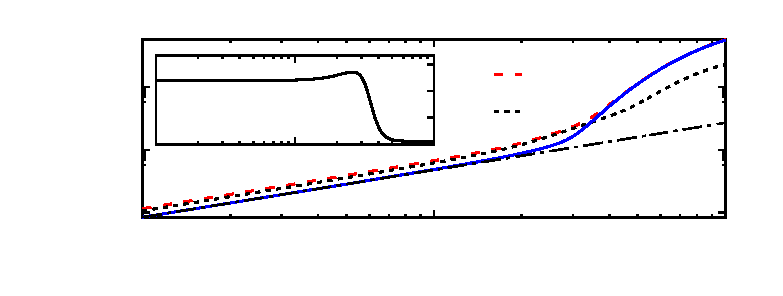
\includegraphics{/home/coelschl/PhD/code/C_Finite_Temp/pics/Ffrc}}%
    \gplfronttext
  \end{picture}%
\endgroup
